%\subsubsection{Hubo2 Plus}
The Hubo2+ is a $1.3\meter$ (4' 3'') tall, 42 $kg$ (93 $lb$) full-size
humanoid robot.  The Hubo series was designed and constructed by the
Korean Advanced Institute of Science and Technology (KAIST) and
spinoff Rainbow Inc. \cite{hubofirst}.  It has 38 degree of freedom:
six per arm and leg, five per hand, three in the neck, and one in the
waist.  Sensors include three-axis force-torque sensors in the wrists
and ankles, accelerometers in the feet, and an inertial measurement
unit (IMU).  The sensors and embedded motor controllers are connected
via a Controller Area Network to a pair of Intel Atom PC104+ PCs
running a GNU/Linux distribution.



% The reference commands for
% all of the joints are sent from the primary control computer (x86) to
% the individual motor controllers via two Controller Area Network (CAN)
% buses.  This is the same communications bus found in most modern motor
% vehicles.  There are currently eight Hubo's functioning in the United
% States as of December 2012.  Four reside at Drexel University and one
% at Georgia Tech, Purdue, Ohio State and MIT.  Jaemi Hubo is the oldest
% of the Hubos in America and has been at the Drexel Autonomous Systems
% Lab\footnote{Drexel Autonomous Systems Lab:
%   http://dasl.mem.drexel.edu/} (DASL) since 2008 \cite{jaemiHuboSRM}.
% Fig.~\ref{fig:hubo} shows the major dimensions of Hubo.

% \begin{figure}[thpb]
%   \centering
% 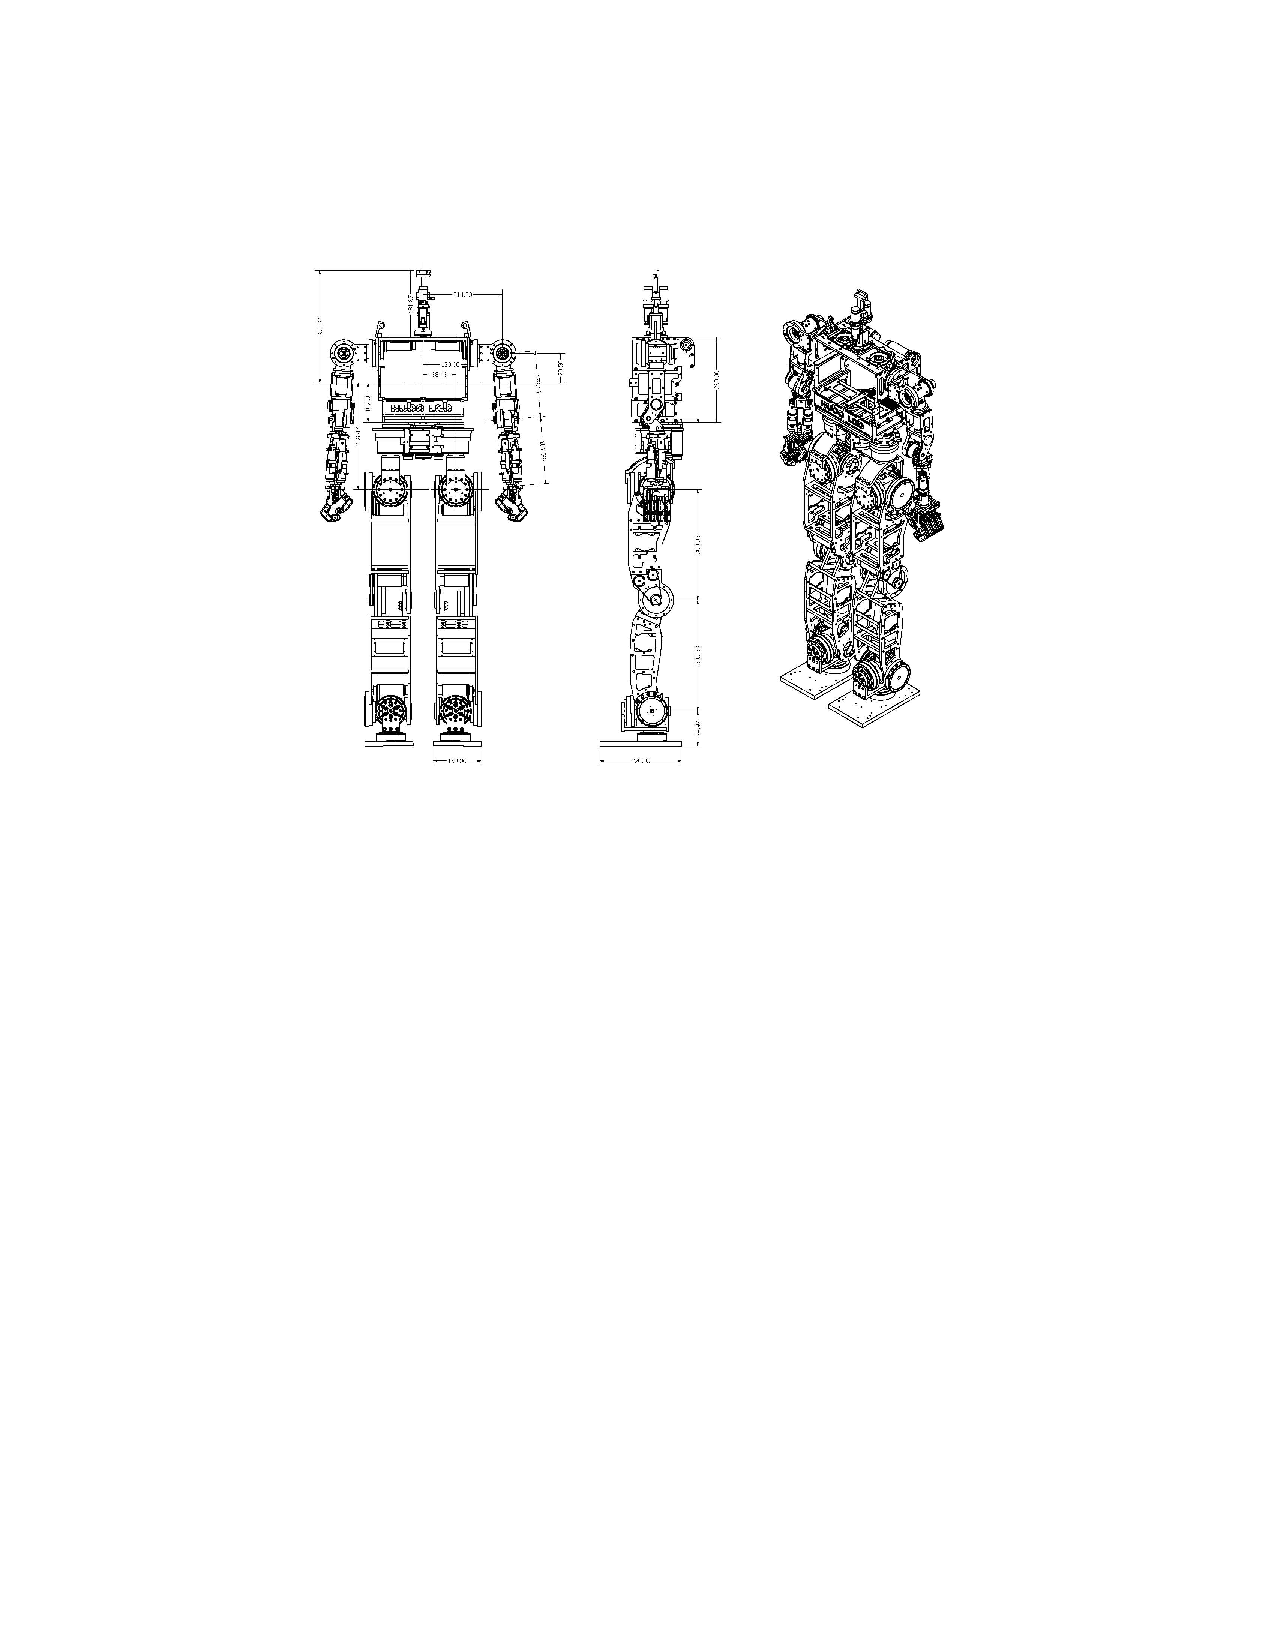
\includegraphics[width=1.0\columnwidth]{./pix/huboSkel.pdf}
%   \caption{Hubo2 Plus platform: 38 DOF, 130 $cm$ tall full-size humanoid robot weighing 37 $kg$.}
%   \label{fig:hubo}
% \end{figure}

% All joints of the major joints are high gain PID position
% controlled with the exception of the fingers.  The fingers are
% open-loop PWM controlled.
% The sensing capability consists of a three
% axis force-torque (FT) sensor on each leg between the end of the ankle
% and the foot as well as between the arm where it connects to the hand.
% Additionally it has an inertial measurement unit (IMU) at the center
% of mass and accelerometers on each foot.

%%% Local Variables:
%%% mode: latex
%%% TeX-master: "ach"
%%% End:
